\documentclass{article}
\usepackage[utf8]{inputenc}
\usepackage{amsmath}
\usepackage{amssymb}
\usepackage{graphicx}
\usepackage{subfig}
\usepackage{tcolorbox}
\usepackage{listings}
\usepackage[left=20mm, right=20mm]{geometry}
\usepackage{enumitem}
\usepackage{amsthm}
\usepackage[hyphens]{url}

\newcommand{\Z}{\mathbb{Z}}
\newcommand{\R}{\mathbb{R}}
\renewcommand{\a}{\land}
\renewcommand{\o}{\lor}
\newcommand{\n}{\neg}
\renewcommand{\i}{\implies}
\newcommand{\p}[1]{\begin{pmatrix} #1\end{pmatrix}}
\newtheorem{theorem}{Theorem}
\newtheorem{lemma}[theorem]{Lemma}

\renewcommand\arraystretch{2}

\title{MATH1061 Assignment 1}
\author{SID: 530328265 - Tutorial\_1: 9.00 WED - Tutorial\_2: 10.00 FRI}
\date{Due Date: 18/3/2024}

\begin{document}
	\maketitle
	\section*{1. }
	\begin{enumerate}[label=({\alph*})]
        \item The condition require for \(\lim_{x\to-2} f(x)\) to exist is:
        \begin{equation}
            \lim_{x\to-2^-} f(x) = \lim_{x\to-2^+} f(x) \quad \label{1:a:1}  
        \end{equation}
        We also have \(\lim_{x\to-2^- f(x)}\), which equals to:\
        \begin{equation}
            \lim_{x\to-2^-} f(x) = \lim_{x\to-2^-} (2 + 2^x) = \lim_{x\to-2^-}(2) + \lim_{x\to-2^-}(2^x) = 2 + 2^{-2} = \frac{9}{4} \quad \label{1:a:2}
        \end{equation}

        From \eqref{1:a:1} and \eqref{1:a:2}, we have \(\lim_{x\to-2^+} f(x)\):
        \begin{align*}
            &\lim_{x\to-2^+} f(x) = \lim_{x\to-2^+} (ax + 1) = \lim_{x\to-2^-} f(x) = \frac{9}{4}\\
            &\Leftrightarrow \lim_{x\to-2^+} (ax + 1) = \frac{9}{4}\\
            &\Leftrightarrow \lim_{x\to-2^+}(ax) + \lim_{x\to-2^+}(1) = \frac{9}{4}\\
            &\Leftrightarrow a(-2) + 1 = \frac{9}{4}\\
            &\Leftrightarrow a = \frac{-5}{8} \quad \blacksquare\\    
        \end{align*}
        
        Thus, The value of a is require for \(\lim_{x\to-2} f(x)\) to exist is \(\frac{-5}{8}\)

        \item Let c \(\in \mathbb{R}\) (The domain of the function). \(f(x)\) is a continious function if and only if \(f(c)\) is define, \(\lim_{x \to c}(f(x))\) exists and is finite, and \(\lim_{x \to c}(f(x)) = f(c)\). 
        % Because \(f(x)\) is a continious function, so we have this property:
        % \[\forall x_{0} \in \mathbb{R}, \lim_{x \to x_{0}} f(x) = f(x_{0}), \text{with } \mathbb{R} \text{ is the domain of the function}\]
        
        Because \(-2 \in \mathbb{R}\) and \(1 \in \mathbb{R}\) so we have:
        % \[\lim_{x \to -2}(f(x)) \text{ exists and equal to } f(-2) \]
        % \[\lim_{x \to 1}(f(x)) \text{ exists and equal to } f(1)\]
 

        \begin{equation}
            \lim_{x \to -2}(f(x)) \text{ exists and equal to } f(-2) \quad \label{1:b:1}
        \end{equation}
        \begin{equation}
            \lim_{x \to 1}(f(x)) \text{ exists and equal to } f(1) \quad \label{1:b:2}
        \end{equation}

        From \eqref{1:b:1}, we have:
        \begin{align*}
            &\lim_{x\to-2^-} f(x) = \lim_{x\to-2^+} f(x) = \lim_{x\to-2} f(x) = f(-2)\\
            &\Leftrightarrow \lim_{x\to-2^+} (ax + 1) = \lim_{x\to-2^-} (2 + 2^x) = 2 + 2^{-2} = \frac{9}{4}\\
            &\Leftrightarrow \lim_{x\to-2^+} (ax + 1) = \frac{9}{4}\\
            &\Leftrightarrow a\times(-2) + 1 = \frac{9}{4}\\
            &\Leftrightarrow a = \frac{-5}{8} \quad \blacksquare\\    
        \end{align*}


        From \eqref{1:b:2}, we have:
        \begin{align*}
            &\lim_{x\to1^-} f(x) = \lim_{x\to1^+} f(x) = \lim_{x\to1} f(x) = f(1)\\
            &\Leftrightarrow \lim_{x\to 1^+} (\frac{c - 2x}{x}) = \lim_{x\to 1^-} (\frac{-5}{8}(x) + 1) = \frac{-5}{8}\times 1 + 1 = \frac{3}{8}\\
            % &\Leftrightarrow  b = \frac{3}{8} \text{ (Because f(x) = b if and only if x = 1)} \quad \blacksquare\\
            &\Leftrightarrow \lim_{x\to 1^+} (\frac{c - 2x}{x}) = \frac{3}{8}\\
            &\Leftrightarrow \frac{c - 2}{1} = \frac{3}{8} \\
            &\Leftrightarrow c = \frac{19}{8} \quad \blacksquare\\
        \end{align*}

        Because \(1 \in \mathbb{R}\), we have:
        \begin{align*}
            \lim_{x \to 1}f(x) &= f(1) \\  
        \end{align*}

        At the same time, \(\lim_{x \to 1}f(x) = \frac{3}{8}\) and \(f(x) = b\) if and only if \(x = 1\) so we have:
        \[f(1) = b = \frac{3}{8} \quad \blacksquare\]

        Thus, If \(f(x)\) is a continious function \(a = \frac{-5}{8}\), \(b = \frac{3}{8}\), \(c = \frac{19}{8}\)

        \item
        \begin{align*}
            \lim_{x \to -\infty} f(x) &= \lim_{x \to -\infty} (2 + 2^x)\\
                                    &= \lim_{x \to -\infty} (2) + \lim_{x \to -\infty}(2^x)\\
                                    &=  2 + 0\\
                                    &= 2\\
        \end{align*}
        \begin{align*}
            \lim_{x \to \infty} f(x) &= \lim_{x \to \infty} (\frac{c - 2x}{x})\\
                                    &= \lim_{x \to \infty} (\frac{\frac{c}{x} - \frac{2x}{x}}{\frac{x}{x}}) \\
                                    &= \lim_{x \to \infty} (\frac{\frac{c}{x} - 2}{1}) \\
                                    &= \lim_{x \to \infty} (\frac{c}{x} - 2) \\
                                    &=  \lim_{x \to \infty} (\frac{c}{x}) - \lim_{x \to \infty} (2) = 0 - 2\\
                                    &= -2    \\
        \end{align*}
	\end{enumerate}

    \newpage
    \section*{2.}
    `\begin{enumerate}[label=({\alph*})]
        \item 
        \[g: D \to \mathbb{R}\text{, } g(x) = \sqrt{\frac{1}{2} + \sin{x}} \text{, which is define if and only if:}\]
        \begin{align*}
            \frac{1}{2} + \sin{x} &\geq 0\\
            \Leftrightarrow \sin{x} &\geq \frac{-1}{2}\\
        \end{align*}


        \begin{figure}[ht]
			\centering
				 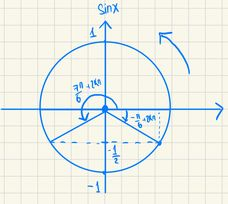
\includegraphics[width=0.4\textwidth]{circle.jpg} 
				 \caption{Ex: 2a}
				 \label{Ex:2a}
		\end{figure}

        As we can see in Figure 1, we can see that:
        \begin{equation}
            \sin{x} = \frac{-1}{2} \leftrightarrow x = \frac{-\pi}{6} + 2k\pi \text{ or } x = \frac{7\pi}{6} + 2k\pi \quad \label{2:a:1}  
        \end{equation}

        
        From Figure 1 and \eqref{2:a:1}, we can find \(D \text{ of } g(x)\)


        This condition holds for some integer \(k \in \mathbb{Z}\)
        \begin{equation}
            \frac{-\pi}{6} + 2k\pi \leq x \leq \frac{7\pi}{6} + 2k\pi
        \end{equation}

        Thus, the natural domain of \(g(x)\) is:
        \[D = [\frac{-\pi}{6} + 2k\pi, \frac{7\pi}{6} + 2k\pi] \text{, with k \(\in \mathbb{Z}\)}\]

        \item
        
        With the natural domain of \(g(x)\), we can see that:
        \begin{align*}
            \frac{-1}{2} &\leq \sin{x} \leq 1\\
            0 & \leq \frac{1}{2} + \sin{x} \leq \frac{3}{2}\\
            \sqrt{0} & \leq \sqrt{\frac{1}{2} + \sin{x}} \leq \sqrt{\frac{3}{2}}\\
            0 & \leq g(x) \leq \sqrt{\frac{3}{2}}
        \end{align*}
        
        Thus, the range of \(g\) is \([0, \sqrt{\frac{3}{2}}]\)

        \item

        Let \(a = \sin{x}\), we can see that the function \(h(x)\) will become:
        \[h(x) = \sqrt{\frac{1}{2} + a}\]

        For each unique value of a, the output of \(h(x)\) will vary accordingly.

        Thus, to make \(h(x)\) bijective, \(\sin{x}\) have to be bijective.

        \begin{figure}[ht]
			\centering
				 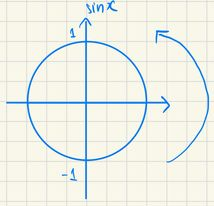
\includegraphics[width=0.4\textwidth]{fig2.jpg} 
				 \caption{Ex: 2c}
				 \label{Ex:2c}
		\end{figure}

        In the Figure 2, we can see that \(\sin{x} \text{ is biject tive }\leftrightarrow  x \in [\frac{-\pi}{2} + 2k\pi, \frac{\pi}{2} + 2k\pi]\), with \(k \in \mathbb{Z}\)

        We can choose only one k to make \(\sin{x}\) bijective. At the same time, we have:
        \[h(0) = \sqrt{\frac{1}{2}}\]
        
        Which means:
         \[0 \in [\frac{-\pi}{2} + 2k\pi, \frac{\pi}{2} + 2k\pi]\]

        Thus, we have to choose \(k = 0\), so we have:
        \begin{equation}
            x \in [\frac{-\pi}{2}, \frac{\pi}{2}] \quad \label{2:c:1}
        \end{equation}


        However, to make \(\sqrt{\frac{1}{2} + \sin{x}}\) exists, so:
        \begin{equation}
            x \in [\frac{-\pi}{6}, \frac{7\pi}{6}] \quad \label{2:c:2}
        \end{equation}

        From \eqref{2:c:1} and \eqref{2:c:2}, the natural domain of \(h(x)\) is:
        \begin{equation}
            x \in [\frac{-\pi}{6}, \frac{\pi}{2}] \quad \label{2:c:3}
        \end{equation}

        Thus, \(\alpha\), \(\beta\) are:

        \begin{equation}
            [\alpha, \beta] = [\frac{-\pi}{6}, \frac{\pi}{2}] \quad \label{2:c:4}
        \end{equation}

        From \eqref{2:c:4} and \(h(x)\) is bijective, \(\gamma\) and \(\delta\) are:
        \begin{equation}
            [\gamma, \delta] = [h(\frac{-\pi}{6}), h(\frac{\pi}{2})] = [0, \sqrt{\frac{3}{2}}]\quad \label{2:c:5}
        \end{equation}

        From, \eqref{2:c:4} and \eqref{2:c:5}, \(\alpha = \frac{-\pi}{6}\), \(\beta = \frac{\pi}{2}\), \(\gamma = 0\) and \(\delta = \sqrt{\frac{3}{2}}\)


        \item
        We have \(h: [\frac{-\pi}{6}, \frac{\pi}{2}] \to [0, \sqrt{\frac{3}{2}}]\text{, } h(x) = \sqrt{\frac{1}{2} + \sin{x}}\)

        \begin{align*}
            y = h(x) &= \sqrt{\frac{1}{2} + \sin{x}}\\
            \Leftrightarrow \sin{x} &= y^2 - \frac{1}{2}\\
            \Leftrightarrow x &= \sin^{-1}{(y^2 - \frac{1}{2})}\\
            \Leftrightarrow h^{-1}(x) &= \sin^{-1}{(x^2 - \frac{1}{2})}\\
        \end{align*}


        As we know, \(h(x)\) is bijective. Thus, domain of \(h(x)\) will be the Co-domain of \(h^{-1}(x)\) and co-domain of \(h(x)\) will be the domain of \(h^{-1}(x)\). Since the domain and the Co-domain of \(h^{-1}(x)\) is:

        \[\text{Domain of } h^{-1}(x) \text{ is: }  [0, \sqrt{\frac{3}{2}}]\]
        \[\text{Co-Domain of } h^{-1}(x) \text{ is: }  [\frac{-\pi}{6}, \frac{\pi}{2}]\]
    \end{enumerate}


        \newpage
        \section*{3. }
        \begin{enumerate}[label=({\alph*})]
            \item
            We have sine function to the complex numbers:
            \[\sin{z}:=\frac{e^{iz} - e^{-iz}}{2i} \text{ for } z \in \mathbb{C}\]

            with \(\sin{z} = -\alpha i \), we have:

            \begin{align*}
                \sin{z} = \frac{e^{iz} - e^{-iz}}{2i} &= - \alpha i\\
                        \Leftrightarrow e^{iz} - e^{-iz} &= -2\alpha i^{2}\\
                        \Leftrightarrow e^{iz} - e^{-iz} &= 2 \alpha\\
                        \Leftrightarrow e^{iz} &=  2\alpha + e^{-iz} \\ 
            \end{align*}
            Using Euler's formula (\(e^{i \alpha} = \cos{\alpha} + i\sin{\alpha}\)), we have:
            \begin{align*}
                 e^{iz} =  2\alpha + e^{-iz} &= 2\alpha + \cos{(-z)} + i\sin{(-z)}\\
                                            &= 2\alpha + \cos{(z)} - i\sin{(z)}\\
                                            &= 2\alpha + \cos{(z)} -\alpha \text{ (Because \(\sin{z} = -\alpha i )\)}\\
                                            &= \alpha + \cos{(z)}
            \end{align*}
        

        We have:
            \[\sin^{2}{x} + \cos^{2}{x} = 1\]
            \[\Leftrightarrow \cos^{2}{x} = 1 - \sin^{2}{x}\]
            \[\Leftrightarrow \cos^{2}{x} = 1 + \alpha^{2}  \text{ (Because \(\sin{z} = -\alpha i )\)}\]
            \begin{equation}
                \Leftrightarrow \cos{x} = \pm \sqrt{1 + \alpha^{2}} \quad \label{3:a:1}
            \end{equation}

            From \eqref{3:a:1}, \(e^{iz}\) equals to:
            \[e^{iz} = \alpha \pm \sqrt{1 + \alpha^{2}} \quad \blacksquare\]


            \item
            Let \(z = a + bi\)
            From a), we have:
            \[e^{iz} = \alpha \pm \sqrt{1 + \alpha^{2}} \text{ with \(\alpha > 1\) and \(\sin{z} = -\alpha i\)}\]
            Then:
            \begin{align*}
                iz &= \ln(a \pm \sqrt{1 + a^{2}})\\
                \Leftrightarrow i(a + bi) &= \ln(a \pm \sqrt{1 + a^{2}})\\
                \Leftrightarrow ai - b &= \ln(a \pm \sqrt{1 + a^{2}})\\
            \end{align*}

            Thus,
            \begin{equation}
                \begin{cases}
                    a &=  0  \quad \quad \quad \quad \quad \quad \quad \quad  \quad \quad \quad \quad \quad \quad \quad \Leftrightarrow \\
                    -b &= \ln(a + \sqrt{1 + a^{2}}) \text{ or } \ln(a - \sqrt{1 + a^{2}}) 
                \end{cases}
                \begin{cases}
                    a &=  0 \\
                    b &= -\ln(a + \sqrt{1 + a^{2}}) \text{ or } -\ln(a - \sqrt{1 + a^{2}}) \quad \label{3:b:1}
                \end{cases}
            \end{equation}
        

        With \(a > 1\) so \(a + \sqrt{1 + a^{2}} > 1\), Thus the first solution \(z \in \mathbb{C}\) is:
        \begin{equation}
            z = a + bi = 0 + (-\ln(a + \sqrt{1 + a^{2}}))i = 0 - \ln(a + \sqrt{1 + a^{2}})i 
        \end{equation}


        We have:
        \begin{align*}
            a^2 &< a^2 + 1 \text{ Because } a > 1\\
            \Leftrightarrow\sqrt{a^{2}} &< \sqrt{a^2 + 1}\\
            \Leftrightarrow a &< \sqrt{a^2 + 1}\\
            \Leftrightarrow a - \sqrt{a^2 + 1} &< 0 \\
        \end{align*}

        However \(ln(x)\) exists if and only if \(x > 0\)

        Thus, it does not exist \(b = -\ln(a - \sqrt{1 + a^{2}})\)

        As a result, we can find only one solution \(z \in \mathbb{C}\) such that \(sin(z) = -\alpha i\), which is:
        \[z = 0 - \ln(a + \sqrt{1 + a^{2}})i \quad \quad \blacksquare\]
        \end{enumerate}

        \newpage
        \section*{4.}

        \begin{enumerate}[label=({\alph*})]
            \item    
            We have \(A = (1,2,3)\), \(B = (-1, 4, 1)\), \(C = (3, 2, -2)\), So \(\overrightarrow{AB}\) and \(\overrightarrow{AC}\) are:

            \[\overrightarrow{AB} =  \begin{bmatrix}x_{B} - x_{A}\\y_{B} - y_{A}\\z_{B} - z_{A}\\\end{bmatrix} = \begin{bmatrix}-1 - 1\\4 - 2\\1 - 3\\\end{bmatrix} = \begin{bmatrix}-2\\2\\-2\\\end{bmatrix}\]
            \[\overrightarrow{AC} =  \begin{bmatrix}x_{C} - x_{A}\\y_{C} - y_{A}\\z_{C} - z_{A}\\\end{bmatrix} = \begin{bmatrix}3 - 1\\2 - 2\\-2 - 3\\\end{bmatrix} = \begin{bmatrix}2\\0\\-5\\\end{bmatrix}\]

            Let \(c_{1}\) and \(c_{2}\) are the coefficients of the linear combination of \(\overrightarrow{AB}\) and \(\overrightarrow{AC}\).

            Thus, we have:
            \begin{align*}
                \textbf{v} &= c_{1}\textbf{\(\overrightarrow{AB}\)} + c_{2}\textbf{\(\overrightarrow{AC}\)}\\
                \Leftrightarrow [k,k - 2,2k - 5] &= c_{1}[-2,2,-2] + c_{2}[2,0,-5]\\
            \end{align*}

            Comparing components gives:

            \begin{equation}
                k = -2c_{1} + 2c_{2} \label{4:a:1}
            \end{equation}
            \begin{equation}
                k - 2 = 2c_{1} + 0c_{2} \label{4:a:2}
            \end{equation}
            \begin{equation}
                2k - 5 = -2c_{1} - 5c_{2} \label{4:a:3}
            \end{equation}
            

            From \eqref{4:a:2}, we have:
            \begin{equation}
                k = 2c_{1} + 2 \label{4:a:4}
            \end{equation}

            From \eqref{4:a:1} and \eqref{4:a:4}, we have:
            \[k = -2c_{1} + 2c_{2} = 2c_{1} + 2\]
            \[\Leftrightarrow 2c_{2}  = 4c_{1} + 2\]
            \[\Leftrightarrow c_{2} = \frac{4c_{1} + 2}{2}\]
            \begin{equation}
                \Leftrightarrow c_{2} = 2c_{1} + 1 \label{4:a:5}
            \end{equation}

            From \eqref{4:a:5} and \eqref{4:a:3}, we have:
            \[2k - 5 = -2c_{1} -5(2c_{1} + 1)\]
            \[\Leftrightarrow 2k - 5 = -12c_{1} -5\]
            \[\Leftrightarrow 2k = -12c_{1}\]
            \begin{equation}
                \Leftrightarrow k = -6c_{1}  \label{4:a:6}
            \end{equation} 
            
            From \eqref{4:a:4} and \eqref{4:a:6}, we have
            \[k = 2c_{1} + 2 = -6c_{1}\]
            \[\Leftrightarrow 8c_{1} = -2\]
            \begin{equation}
                \Leftrightarrow c_{1} = \frac{-2}{8} = \frac{-1}{4} \label{4:a:7}
            \end{equation}

            From \eqref{4:a:7} and \eqref{4:a:6}, we have:
            \begin{equation}
                k = -6 \times \frac{-1}{4} = \frac{3}{2} \label{4:a:8}
            \end{equation}


            From \eqref{4:a:7} and \eqref{4:a:5}, we have:
            \begin{equation}
                c_{2} = 2 \times \frac{-1}{4} + 1 = \frac{1}{2} \label{4:a:9}
            \end{equation}

            From \eqref{4:a:7}, \eqref{4:a:8} and \eqref{4:a:9},we have:
            \[c_{1} = \frac{-1}{4}\]
            \[c_{2} = \frac{1}{2}\]
            \[k = \frac{3}{2}\]

            Thus, \textbf{v} is:
            \[\textbf{v} = [k,k-2,2k-5] = [\frac{3}{2},\frac{-1}{2},-2]\]

            And write \textbf{v} as a linear combination of \(\overrightarrow{AB}\) and \(\overrightarrow{AC}\) is:

            \[[k,k - 2,2k - 5] = c_{1}[-2,2,-2] + c_{2}[2,0,-5]\]
            \[\Leftrightarrow [\frac{3}{2},\frac{-1}{2},-2] = \frac{-1}{4}[-2,2,-2] + \frac{1}{2}[2,0,-5]\]
            \item
            In a), we have:
            \[\overrightarrow{AB} = [-2, 2, -2]\]
            \[\overrightarrow{AC} = [2,0,-5]\]

            \[\overrightarrow{BC} = \begin{bmatrix}x_{C} - x_{B}\\y_{C} - y_{B}\\z_{C} - z_{B}\\\end{bmatrix} = \begin{bmatrix}-3 - (-1)\\2 - 4\\-2 - 1\\\end{bmatrix} = \begin{bmatrix}4\\-2\\-3\\\end{bmatrix}\]

            Then, length of vectors \(\overrightarrow{AB}\), \(\overrightarrow{AC}\) and \(\overrightarrow{CB}\) are:
            \[\|\overrightarrow{AB}\| = \sqrt{(-2)^2 + 2^2 + (-2)^2} = 2\sqrt{3}\]
            \[\|\overrightarrow{AC}\| = \sqrt{(-2)^2 + 0^2 + (-5)^2} = \sqrt{29}\]
            \[\|\overrightarrow{BC}\| = \sqrt{(4)^2 + (-2)^2 + (-3)^2} = \sqrt{29}\]

            We can see that \(\|\overrightarrow{AC}\| = \|\overrightarrow{BC}\|\)
            
            Thus, \(\triangle\)ABC isoceles at vertex C 

            \begin{figure}[ht]
                \centering
                     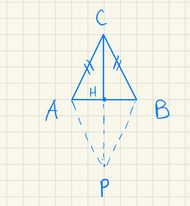
\includegraphics[width=0.4\textwidth]{ex4.jpg} 
                     \caption{Ex: 4b}
                     \label{Ex:4b}
            \end{figure}


            A rhombus is a quadrilateral with all sides of equal length. By definition, the diagonals of a rhombus intersect at their midpoint. Thus, I call H is a middle point of AB, then H also have to be the middle point of CP.

            The coordinate of H is:
            \[H = (\frac{x_{A} + x_{B}}{2}, \frac{y_{A} + y_{B}}{2}, \frac{z_{A} + z_{B}}{2}) = (\frac{1 + (-1)}{2}, \frac{2 + 4}{2}, \frac{3 + 1}{2}) = (0, 3, 2)\]


            Let coordinate of \(P = (x_{P}, y_{P}, z_{P})\). Because H also the middle point of CP, so we have:
            \[H = (0,3,2) = (\frac{x_{C} + x_{P}}{2}, \frac{y_{C} + y_{P}}{2}, \frac{z_{C} + z_{P}}{2}) = (\frac{x_{C} + x_{P}}{2}, \frac{y_{C} + y_{P}}{2}, \frac{z_{C} + z_{P}}{2}) = (\frac{3 + x_{P}}{2}, \frac{2 + y_{P}}{2}, \frac{-2 + z_{P}}{2})\]\

            Thus we have the equation.
            \begin{equation}
                0 = \frac{3 + x_{P}}{2}
            \end{equation}
            \[\Leftrightarrow x_{P} = -3\]
            \begin{equation}
                3 = \frac{2 + y_{P}}{2}
            \end{equation}
            \[\Leftrightarrow y_{P} = 4\]
            \begin{equation}
                2 = \frac{-2 + z_{P}}{2}
            \end{equation}
            \[\Leftrightarrow z_{P} = 6\]


            Thus, coordinate of P is \(P = (-3, 4, 6)\)
        \end{enumerate}
    \end{document}